\documentclass[12pt]{article}

\usepackage{fullpage}
\usepackage{graphics}
\usepackage{tikz}
\usepackage[parfill]{parskip}
\usepackage[utf8]{inputenc}
\usepackage{etoolbox}
\usepackage{ textcomp }

\newbool{alt}
\booltrue{alt}
%\boolfalse{alt}
 
% Standard things to include for math   
\usepackage{amsmath,amssymb,amsfonts,amsthm}

\usepackage{wasysym}

\usepackage{enumitem}



\usepackage{geometry}
 \geometry{
 a4paper,
 top=2cm,
 bottom=2cm,
 left=2cm,
 right=2cm,
 }




% Some of Ebrahim's definitions
\newcommand{\done}{\\\hspace*{0pt}\hfill$\blacksquare$}
\def\N{\mathbb{N}}
\def\R{\mathbb{R}}
\def\Q{\mathbb{Q}}
\def\Z{\mathbb{Z}}
\def\e{\epsilon}
\newcommand{\seq}[1]{\left(#1\right)_{n\in\N}}
\newcommand{\Euc}[1]{\mathbb{R}^{#1}}
\newcommand{\pathvarNaked}{p}
\newcommand{\pathvar}{\vec{\pathvarNaked}}
\newcommand{\pathvarAlt}{\vec{q}}
\newcommand{\exercisesList}[2]{\textcolor{ForestGreen}{Exercises from WeBWorK HW#1: #2.}}
\newcommand{\exerciseText}[1]{\textcolor{ForestGreen}{Exercise: #1}}
\def\vx{\vec{x}}
\def\vu{\vec{u}}
\def\vv{\vec{v}}
\def\vw{\vec{w}}
\newcommand{\der}[2]{\frac{\textrm{d}#1}{\textrm{d}#2}}
\newcommand{\derOp}[1]{\der{\phantom{#1}}{#1}}
\newcommand{\pder}[2]{\frac{\partial #1}{\partial #2}}
\newcommand{\pderOp}[1]{\pder{\phantom{#1}}{#1}}
\newcommand{\colvectwo}[2]{\left[\begin{array}{c}#1\\#2\end{array}\right]}
\newcommand{\colvectwoXYVEC}[2]{\left[#1\right]\,\cbv{x} + \left[#2\right]\,\cbv{y}}
\newcommand{\colvecthree}[3]{\left[\begin{array}{c}#1\\#2\\#3\end{array}\right]}
\newcommand{\colvecfour}[4]{\left[\begin{array}{c}#1\\#2\\#3\\#4\end{array}\right]}
\newcommand{\colvecfourL}[4]{\left[\begin{array}{l}#1\\#2\\#3\\#4\end{array}\right]}
\newcommand{\norm}[1]{\left|\hspace{-1.5pt}\left|#1\right|\hspace{-1.5pt}\right|}
\def\grad{\vec{\nabla}}
\newcommand{\Dir}[3]{\operatorname{Dir}(#1,#2,#3)}
\newcommand{\D}[1]{\textrm{D}#1}
\def\vn{\vec{n}}
\newcommand{\cbv}[1]{\partial_{#1}}
\newcommand{\arrayBrackets}[2]{\left[ \begin{array}{#1} #2 \end{array} \right] }

\makeatletter
\newcommand*\dotp{\mathpalette\bigcdot@{.5}}
\newcommand*\bigcdot@[2]{\mathbin{\vcenter{\hbox{\scalebox{#2}{$\m@th#1\bullet$}}}}}
\makeatother



\newcommand{\ansbox}[2]{\raisebox{-.5\height}{\framebox(#1,#2){}}}

\def\endans{\hspace{1em}\ansbox{40}{40}}


\newcommand{\NEcheckbox}{ % Put check box on northeast corner of page
\begin{tikzpicture}[remember picture,overlay] 
\path (current page.north east) ++(-1,-1) node[below left] {
{\small graded?} {\Large\Square}
};
\end{tikzpicture}
}

\newcommand{\LEFTcheckbox}{ % Put check box in the left margin
\\\begin{tikzpicture}[remember picture,overlay] 
\path ++(-2,0) node[below left] {
 {\Large\Square}
};
\end{tikzpicture}
}

\newcommand{\LEFTcheckboxOwnLine}{ % Put check box in the left margin, use this one if on own line
\begin{tikzpicture}[remember picture,overlay] 
\path ++(-2,0) node[below left] {
 {\Large\Square}
};
\end{tikzpicture}
}






\pagenumbering{gobble}
\begin{document}




% --- Score table ---

%\def\gap{\hspace*{2.5em}}
%
%\begin{tikzpicture}[overlay, remember picture]
%\path (current page.north east) ++(-1,-1) node[below left] {
%\begin{tabular}{c|c|c|c|c|c|c|c}
% 1 &  2 & 3 & 4 & 5 & 6 & 7 & $\Sigma$\\ \hline
% \gap & \gap & \gap & \gap & \gap & \gap & \gap & \gap \\
% \gap & \gap & \gap & \gap & \gap & \gap & \gap & \gap
%\end{tabular}
%};
%\end{tikzpicture}

% ---


\def\namepos{(current page.north west) ++(5,-0.8)}
\begin{tikzpicture}[overlay, remember picture]
\draw [black] \namepos rectangle ++(10,-1);
\draw [black] \namepos ++(0,-1.2) rectangle ++(10,-1);
%\draw [black] \namepos ++(0,-1.2) ++(0,-1.2) rectangle ++(10,-1);
%\draw [black] \namepos ++(0,-1.2) ++(0,-1.2) ++(0,-1.2) rectangle ++(10,-1);
\path \namepos ++(0,-0.4) node [left] {\textbf{Name:}};
\path \namepos ++(0,-0.4) ++ (0,-1.2) node [left] {\textbf{Perm:}};
%\path \namepos ++(0,-0.4) ++ (0,-1.2) ++ (0,-1.2) node [left] {\textbf{Seat Number:}};
%\path \namepos ++(0,-0.4) ++ (0,-1.2) ++ (0,-1.2) ++ (0,-1.2) node [left] {\textbf{ID Checker Name:}};
\end{tikzpicture}

\def\versionRowText{
\textit{version \ifbool{alt}{1}{2},row}
\raisebox{-3pt}{\framebox(15,15){A}}
}
\begin{tikzpicture}[overlay, remember picture]
\path (current page.north east) ++ (-2,-1.5) node [left] %{\versionRowText};
\end{tikzpicture}



\vspace{5em}

\begin{center}\textbf{Math 34A Final Exam, Spring 2022}\end{center}

\begin{enumerate}
\newpage
\phantom{.}
%%%%%%%%%%% (1)
\newpage
\item ({\it 15 pts}) Please use the graph below to estimate your answers. \\
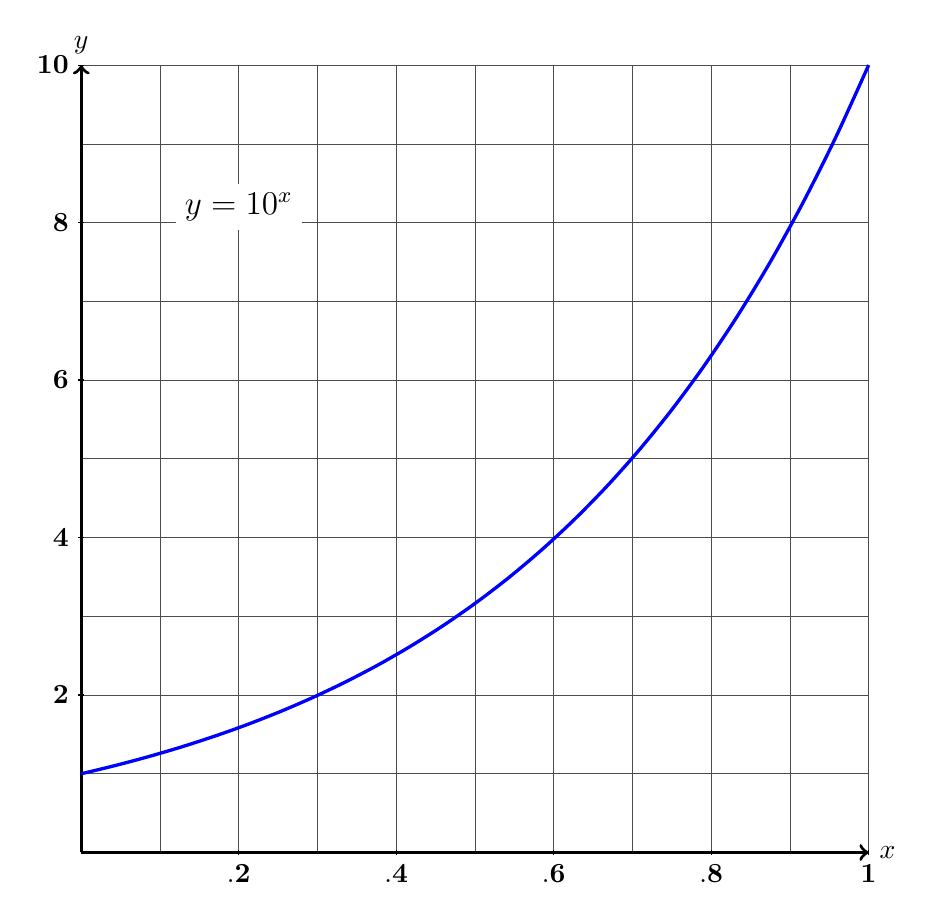
\begin{tikzpicture}
 %grid
  \draw[step=1cm,black!70,very thin] (0,0) grid (10,10);
  %axes
  \draw[very thick,->] (0,0) -- (10,0) node[anchor= west] {\bf{$x$}};
  \draw[very thick,->] (0,0) -- (0,10) node[anchor=south] {\bf{$y$}};
  \foreach \x in {.2,.4,.6,.8,1}
    \draw (10*\x cm,1pt) -- (10*\x cm,-1pt) node[anchor=north] {$\mathbf{\x}$};
  \foreach \y in {2,4,6,8,10}
    \draw (1pt,\y cm) -- (-1pt,\y cm) node[anchor=east] {$\mathbf{\y}$};
   %Function Name
   \node[black,fill=white] at (2,8.2)
   {{\large $y=10^x$}};
   %function
   \draw[scale=1.0,domain=0:10,smooth,variable=\x,blue,very thick] plot (\x,{10^(.1*\x)})
   %Code from previous exam below:
   %\draw[thick,black] plot[domain=0:10] (\x,{10^(.1*\x)})
   ;
 \end{tikzpicture}
\begin{enumerate} 
\item Find $\log(2512)$ 
\vfill
\phantom{.} \hfill$\log(2512) \approx \ $ \ansbox{100}{60} 
\item Find $\log(2^{10})$ 
\vfill
\phantom{.} \hfill$\log(2^{10}) \approx \ $ \ansbox{100}{60} 
\item Approximate a solution for $x$ in the equation $2^{3x-5}=5^3$ 
\vfill
\phantom{.} \hfill$x \approx \ $ \ansbox{100}{60} 
%\item Using the approximation in your previous answer as well as the fact that $2^{10}$ is exactly 1024, compare the two values by writing a $<$, $=$ or $>$ in the box below. \\ 
%If you are stuck, consider taking the anti-log of both numbers in part (b). 
%\vfill
%\phantom{.} \hfill$\log(2) \ $ \ansbox{40}{40} $ \ .3$
\end{enumerate} 




\newpage
%%%%%%%%%%% (2)
\item ({\it 6 pts}) For this problem, $k$, $m$, and $b$ are constant values. Find $\displaystyle\frac{d}{dx}\left( 2ke^{3kx} + mx + b \right)$ and simplify your answer. \\
\vfill \\
$\displaystyle\frac{d}{dx}\left( 2ke^{3kx} + mx + b \right)=$ \ansbox{300}{70} \vspace{20pt} 


%%%%%%%%%%% (3)
\item ({\it 10 pts}) This question is about the graph of the function
$$f(x)=-x^2 + 8x + 16.$$
\begin{enumerate} 
\item When does $f$ achieve its highest value? \\ 
\vfill \\
\phantom{.} \hfill When $x= \ $ \ansbox{100}{70} 
\item Write the equation of the tangent line at $x=0$ in the form $y=mx+b$. \\ 
\phantom{.} \hfill$  y=  $ \ansbox{240}{70} 
\end{enumerate}


\newpage
%%%%%%%%%%% (4)
\item ({\it 7 pts}) For each part of problem (4) please use the graph below to estimate your answers. \\
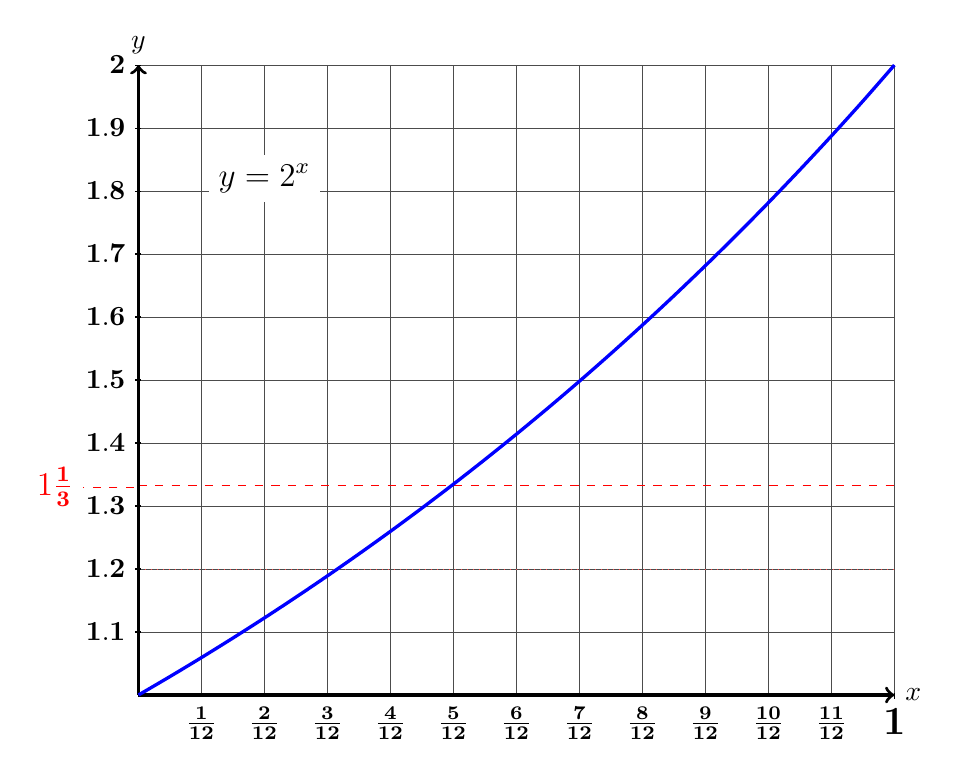
\begin{tikzpicture}[scale=.8]
 %grid
  \draw[step=1cm,black!70,very thin] (0,0) grid (12,10);
  %extra dotted line
  \draw[red, dashed] (0,3.33) -- (12,3.33);
  \draw[step=1cm,red!70,very thin, dotted] (0,1.3333) grid (12,1.3333);
  %axes
  \draw[very thick,->] (0,0) -- (12,0) node[anchor= west] {\bf{$x$}};
  \draw[very thick,->] (0,0) -- (0,10) node[anchor=south] {\bf{$y$}};
  \foreach \x in {1,2,3,4,5,6,7,8,9,10,11}
    \draw (\x cm,1pt) -- (\x cm,-1pt) node[anchor=north] {$\frac{\mathbf{\x}}{\mathbf{12}}$};
    \draw (12 cm,1pt) -- (12 cm,-1.8pt) node[anchor=north] {{\Large $\mathbf{1}$}};
  \foreach \y in {1.1,1.2,1.3,1.4,1.5,1.6,1.7,1.8,1.9,2}
    \draw (1pt,10*\y cm -10cm) -- (-1.5pt,10*\y cm -10cm) node[anchor=east] {$\mathbf{\y}$};
   \draw[dashed, red] (-2pt,10*1.33 cm -10cm) -- (-25pt,10*1.33 cm -10cm) node[anchor=east] {\small{\large{$1\frac{\mathbf{1}}{\mathbf{3}}$}}};
   %Function Name
   \node[black,fill=white] at (2,8.2)
   {{\large $y=2^x$}};
   %function
   \draw[scale=1.0,domain=0:12,smooth,variable=\x,blue,very thick] plot (\x,{2^(\x/12)*10-10})
   %Code from previous exam below:
   %\draw[thick,black] plot[domain=0:10] (\x,{10^(.1*\x)})
   ;
 \end{tikzpicture}
\begin{enumerate} 
\item ({\it 3pts}) Find a solution for $2^x = \frac{4}{3}$\\
\phantom{.} \hfill$x \approx \ $ \ansbox{100}{90} 

\item ({\it 4pts}) The SoCal Burger restaurant chain has been very popular since they first opened their first location in Santa Barbara a few years ago and they now have hundreds of locations. In fact, over the last twelve months the number of locations has doubled! In order to set a world record, they just need to grow 50\% over the next year. Assuming that their steady, exponential growth from last year continues over the next year, how many months would it take? \\
(Hint, the answer is {\bf not} 6 months). \\ \\ 
A model that might be helpful: $y=A\cdot2^t$,
where $y$ is the number of locations $t$ years from now and $A$ is the current number of locations. \\
\vfill
\phantom{.} \hfill$\approx \ $ \ansbox{100}{70} months


\end{enumerate}




\newpage
%%%%%%%%%%% (5)
\newpage
\item ({\it 9pts}) Below is the graph of a funtion $g(x)$ with five labeled points, $A$, $B$, $C$, $D$, and $E$. Identify a point where $g''(x) < 0$, a point where $g''(x) = 0$, and a point where $g''(x) > 0$. \vspace{10pt} \\ 

%f(x)=0.02 (x+4) (x+2) x (x-2) (x-4) for the graph below in Geogebra
\fbox{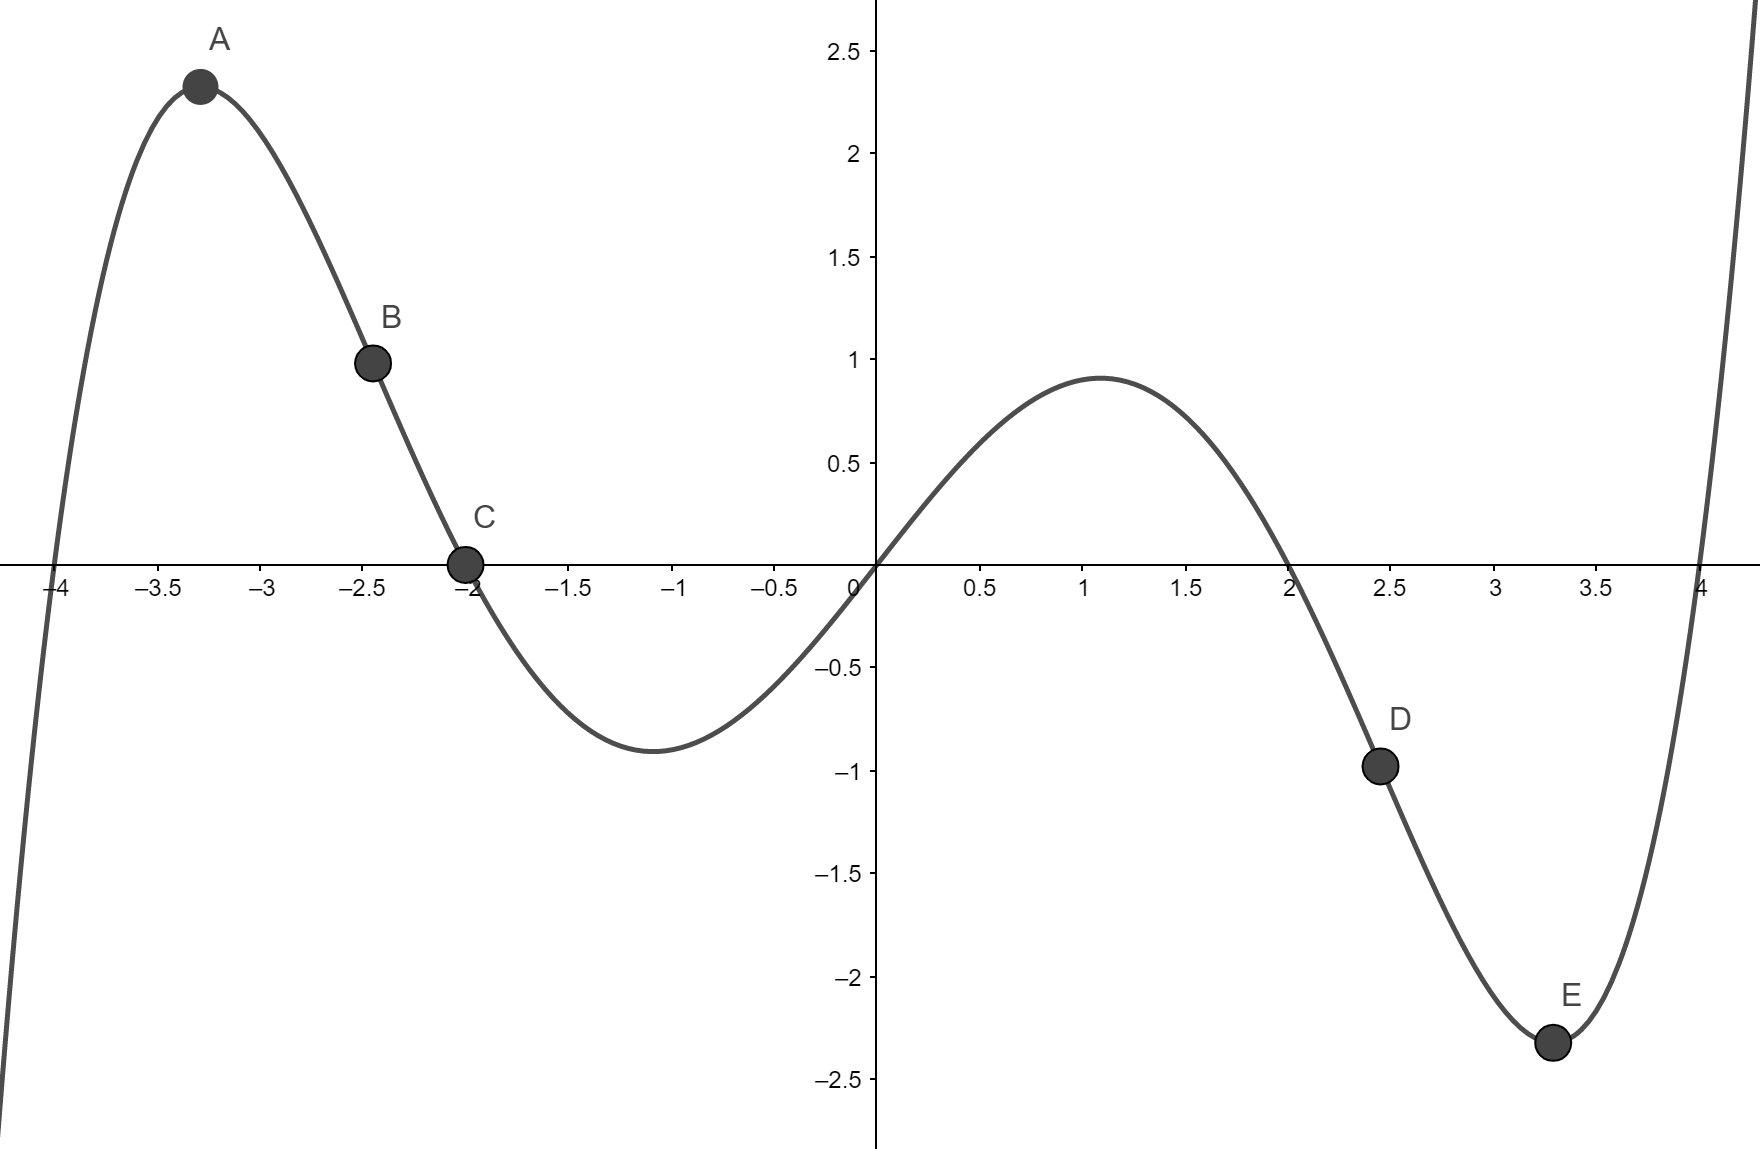
\includegraphics[scale=.45]{Final_Exam_Graph_Black.png}} \\
\vspace{15pt}\\
    \phantom{.} \hfill 
     \begin{tabular}{C C C}
     \ansbox{60}{50} \ & \ \ansbox{60}{50} & \ansbox{60}{50} \\
     $g''(x) < 0$ & $g''(x) = 0$ & $g''(x) > 0$
     \end{tabular}
     
    
    

%%%%%%%%%%% (6)
\item ({\it 10pts}) For this problem, $f(x) = (x^2+3)(x+2).$ \vspace{20pt}
\begin{enumerate} 
\vfill
\item $f'(x)=$\phantom{.} \ansbox{400}{70} \vspace{20pt} %\\
\vfill
\item $f''(x)=$ \ansbox{400}{70} \vspace{20pt} %\\
\end{enumerate}




	
	
    
    
\newpage
%%%%%%%%%%% (7)    
\item ({\it 15pts}) Jack Johnson* will be playing at the Santa Barbara Bowl next fall. He gives you 100 concert tickets, asking you to sell them on campus for a charity and to give away any left-over tickets. The price is up to you, but you need to sell them all at the same price. If the price you set is \$20 each then you would sell all 100 tickets. For each dollar you decide to increase the price, the number of tickets you could sell would decrease by 2. 
\begin{enumerate}
\item If your ticket price is
$\$(20 + x)$, how many tickets would you be able to sell? \\ 
\vspace{30pt} \\
\phantom{.} \hfill  \ansbox{150}{50} tickets
\item What is the total amount of
money (in terms of $x$) you would receive for selling those tickets? You do not need to simplify your answer for this part. \\ 
\vfill
\phantom{.} \hfill {\Large \$} \ \ansbox{350}{50} 
\item What is the maximum amount of money you could receive from selling tickets? \\ 
\vfill
\vfill
\vfill
\phantom{.} \hfill {\Large \$} \ \ansbox{80}{50} 
\end{enumerate}
\scriptsize{*Maybe this story isn't so far-fetched. Jack Johnson is a UCSB alumnus and after he heard about a tragic event that happened here a few years ago he came and played a free concert in front of Storke Tower. He also fund-raises frequently for people in need in this area, including a benefit a couple months ago for victims of the Thomas fire.} 


%    \newpage
%    \phantom{.}













\end{enumerate}



\end{document}

